\documentclass[12pt]{article}
% Font family
\usepackage{xeCJK}
\setCJKmainfont{Noto Serif TC}
\usepackage{amssymb}
\usepackage{amsmath}

% Document layout
\usepackage[margin=2cm, a4paper]{geometry}
\usepackage{setspace}
\onehalfspacing
\setlength{\parskip}{12pt}
\setlength{\parindent}{0pt}

% Citation
\usepackage{biblatex}
\addbibresource{./ref.bib}

% Image
\usepackage{graphicx}
\graphicspath{{./images/}}

\author{\normalsize 施宇庭 NN6124030}
\date{}


\title{\Large AOC 2024 Spring - Lab 2 Quantization}

\begin{document}
\maketitle

\section{Implementation of Quantization Functions}

\subsection*{Q1}
\begin{figure}[h]
    \centering
    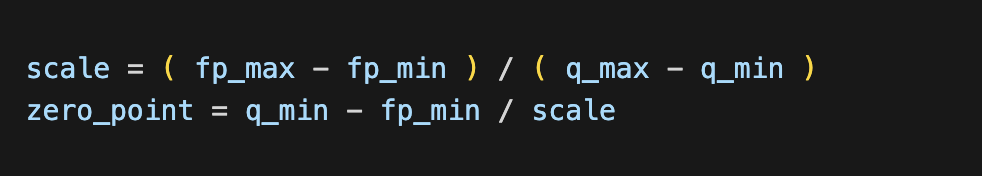
\includegraphics[width=0.9\linewidth]{./images/lab2_q1.png}
    \caption{Scale and zero point.}
\end{figure}

\subsection*{Q2}
\begin{figure}[h]
    \centering
    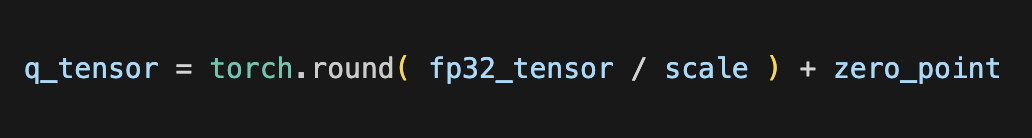
\includegraphics[width=0.9\linewidth]{./images/lab2_q2.png}
    \caption{Quantizating a tensor from FP32 to INT8.}
\end{figure}

\subsection*{Q3}
\begin{figure}[h]
    \centering
    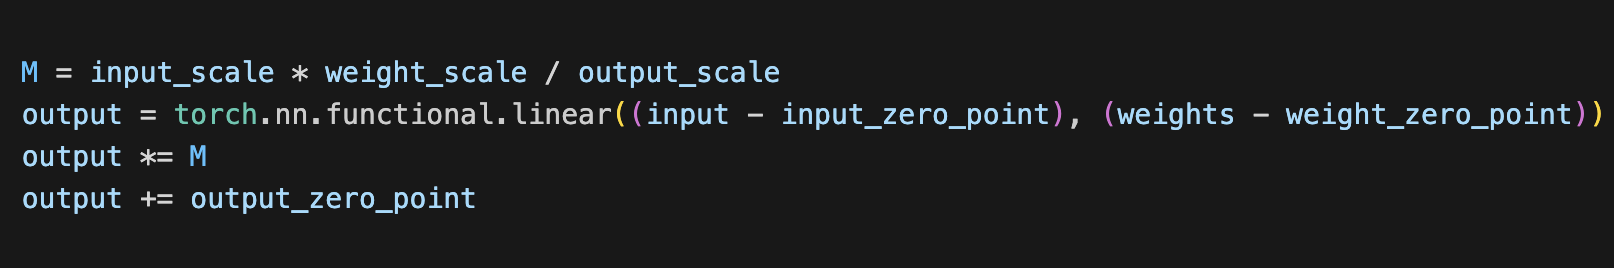
\includegraphics[width=0.9\linewidth]{./images/lab2_q3.png}
    \caption{Quantized linear layer.}
\end{figure}

\section{Problems}

\subsection{Quantized Model Size Evaluation}
% What is the size of the model after int8 quantization if its original size is 50MB?
% Please write down your calculation process. (Assume the original resolution is 32 bits) (15%)

Assume that the data type of all the parameters in the original full-precision model are FP32.
The number of parameters is $50\text{MB} \div 4\text{B} = 12.5\text{M}$, and the size of each INT8 parameter is $1\text{B}$.
Therefore, the size of quantized model is $12.5\text{M} \times 1\text{B} = 12.5\text{MB}$.

\subsection{Scaling Factor of Quantization}
% If M = 0.2, determine values for M0 and n such that the equation on page 11 is true. (10%)

If $M = 0.2$, then $M_0 = 0.8$ and $n = 2$.

\subsection{Software/Hardware Co-design for Quantization}

\subsubsection{Normalization of the Scale Multiplier for Fixed-Point Arithmetic}

論文中有提到 scale multiplier $M$ 通常介於 (0, 1) 之間,為了能夠使用定點數取代浮點數運算,並最大程度保留 $M_0$ 的精度 (小數點後的位數),因此有以下定義:

\begin{equation}
M = 2^{-n} M_0
\label{eq:1}
\end{equation}
$$
\text{where } M \in \mathbb{R} \text{, } M_0 \in [0.5, 1) \text{, and } n \in \mathbb{N} \cup \{0\}
$$

而 $M_0$ 的整數表示法則為以下式子,其中 $\lfloor \cdot \rceil$ 表示 round to nearest

\begin{equation}
\text{IntRepr}(M_0) = \lfloor 2^{B-1} M_0 \rceil
\label{eq:2}
\end{equation}

定義中 $M_0$ 位於 $[0.5, 1)$ 之間,也就是二進位的 $[0.1_2, 1_2)$ 之間,如果用 int8 ($B = 8$) 來表示 $M_0$,則其整數表示法的二進位則為 $[01000000_2, 10000000_2)$,除了最高和次高位元以外的 6 bits 都可以拿來表示小數部分。

假設 $M = 0.064453125 = 0.000100001_2$,若不將 $M$ normalize 成 $M_0$,其 int8 整數表示法的二進位為 $00010000_2$,和 $0.0625 (= 0.0001_2)$ 的整數表示法 $00010000_2$ 一模一樣,經歷了精度損失。但如果依照上述公式將 $M$ normalize 成 $M_0$ ($n=3$),則 $0.064453125$ 將表示為 $01000010_2$,$0.0625$ 則表示為 $01000000_2$,兩者可以區分開來。

且根據 Eq. \eqref{eq:1},從 $M_0$ 計算 $M$ 時,可以向右位移 $n$ bits 來得到。

\subsubsection{Hardware Implementation for Fixed-Point Multiplication}

依照論文的描述 $M_0$ 通常會選擇用 int16 或 int32 的資料型態,依照 Eq. \eqref{eq:2},會用 1 bit 來表示整數部分,其餘的 bits 表示小數部分,再做無號整數乘法,最後取整數部分最低位的 1 bit,以及小數部分的高位 15 bits 或 31 bits。

\begin{figure}[h]
    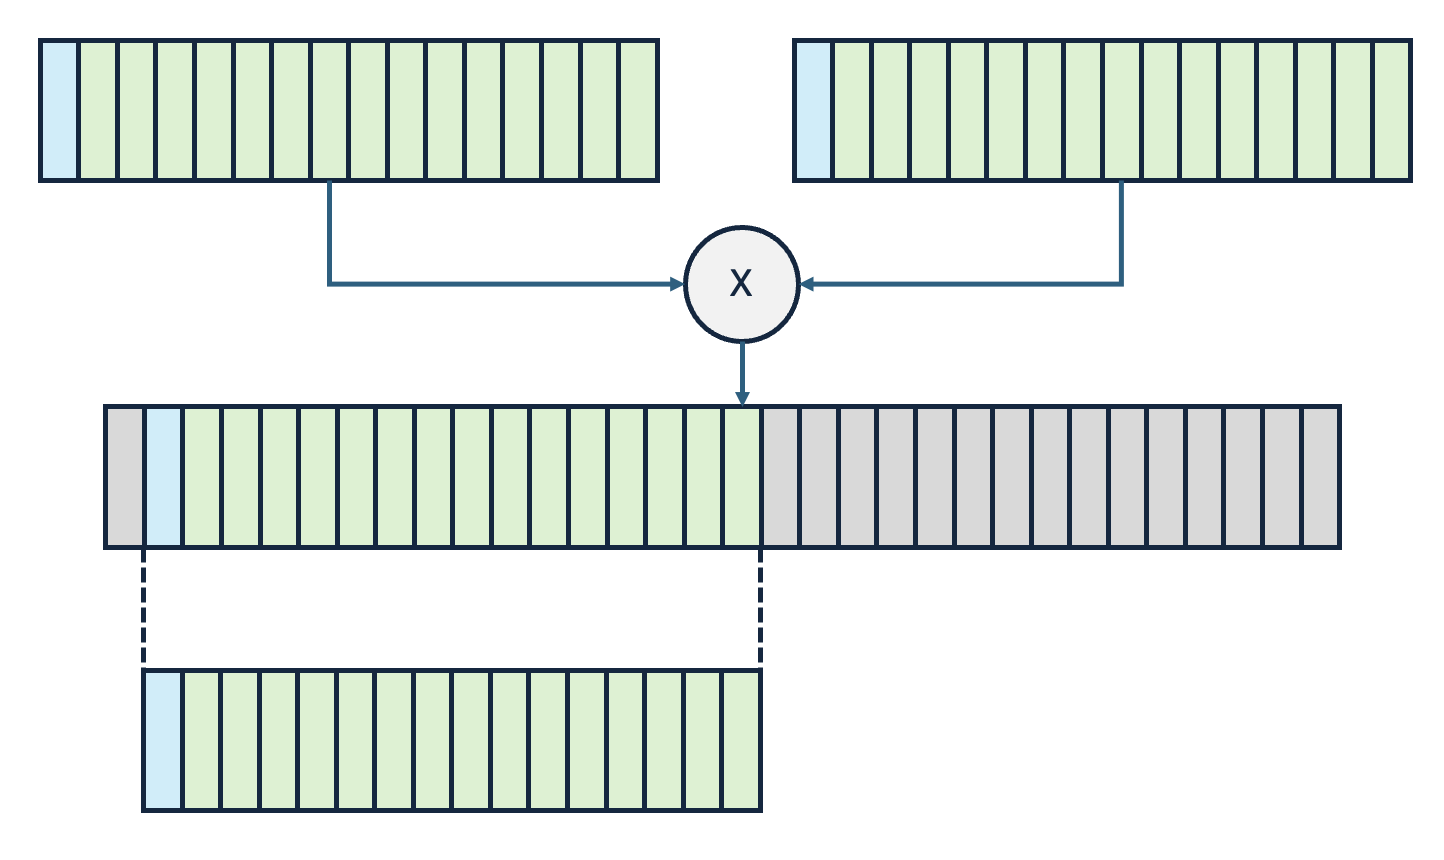
\includegraphics[scale=0.5]{./fixed-point-mul.png}
    \centering
    \caption{16-bit fixed-point multplication}
\end{figure}

% 1. fixed-point multiplication by a normalized multiplier $M_0$

% 2. rounding bit-shift

% 3. saturating cast to uint8

\subsubsection{Hardware Implementation for Saturation}

Saturation 的操作可以表示為以下函數:

$$
\text{Saturate}(x) = \min(\max(x, a), b)
$$

其中 $a$ 和 $b$ 分別是量化後數值的最小值和最大值,例如使用 uint8 來表示量化後的數值的話,則 $a=0$、$b=255$。

硬體的實現可以用兩個比較器 (comparator) 和兩個多工器 (multiplexer, mux) 來達成,用比較器輸出作為多工器的控制訊號,來決定最終要輸出 $x$、$a$ 或 $b$,以下為 Verilog 的實作:

\begin{verbatim}
module Saturator #(
    parameter IN_WIDTH = 32,
    parameter OUT_WIDTH = 8,
    parameter MIN = 0,
    parameter MAX = 255
) (
    input [IN_WIDTH-1:0] in,
    output [OUT_WIDTH-1:0] out
);
    assign out = (in < MIN) ? MIN :
                 (in > MAX) ? MAX :
                 in[OUT_WIDTH-1:0];
endmodule
\end{verbatim}

另外,由於本篇論文最後會 cast 成 uint8 的資料型態,最小值一定是 0,最大值一定是 255,所以可以再簡化成以下這樣,只需要一個比較器和兩個 mux。

\begin{verbatim}
    module Saturator #(
        parameter IN_WIDTH = 32,
        parameter OUT_WIDTH = 8,
    ) (
        input [IN_WIDTH-1:0] in,
        output [OUT_WIDTH-1:0] out
    );
        assign out = (in[IN_WIDTH-1]) ? 8'd0 :
                     (in > MAX) ? 8'hff :
                     in[OUT_WIDTH-1:0];
    endmodule
    \end{verbatim}

\subsubsection{Batch Normalization Folding}

Batch normalization

$$
\hat x_i = \gamma \frac{x_i - \mu}{\sqrt{\sigma^2 + \epsilon}} + \beta
= \frac{\gamma x_i}{\sqrt{\sigma^2 + \epsilon}} - \frac{\gamma \mu}{\sqrt{\sigma^2 + \epsilon}} + \beta
$$

$$
\text{where } \mu = \frac{1}{n}\sum_{i=1}^{n}x_i
\text{, }
\sigma = \frac{1}{n} \sum_{i=1}^{n} (x_i - \mu)^2
$$

其中 $\mu$ 和 $\sigma^2$ 是 input activation 在 batch 方向的平均值和變異數,訓練時會從 training 資料集中計算出來, testing 時則使用 exponential moving avarage 來反映測試資料的分布狀況。
$\gamma$ 和 $\beta$ 則是 learnable 的參數,會在 training 時藉由 gradient descent 從 training data 中計算出來,在 testing 時則固定不動。

%由於 batch normalization 是對 N, H, W 方向進行 normalization,也就是一個 N*C*H*W 的 input feature map 會算出 C 個平均值和變異數,

由於 convolution 可以表示成矩陣乘法 (GEMM)
$$
\mathbf{O}_\text{conv} = \mathbf{W}_\text{conv} \cdot \mathbf{I}_\text{conv} + \mathbf{b}_\text{conv}
$$

batch normalization 也可以表示成 GEMM
$$
\mathbf{O}_\text{bn} = \mathbf{W}_\text{bn} \cdot \mathbf{I}_\text{bn} + \mathbf{b}_\text{bn}
$$

因此兩個操作可以合併在一起,在 inference 時只要做一次 GEMM 即可

\begin{align*}
\mathbf{O}_\text{bn} &= \mathbf{W}_\text{bn} \cdot (\mathbf{W}_\text{conv} \cdot \mathbf{I}_\text{conv} + \mathbf{b}_\text{conv}) + \mathbf{b}_\text{bn} \\
&= (\mathbf{W}_\text{bn} \cdot \mathbf{W}_\text{conv}) \cdot \mathbf{I}_\text{conv} + (\mathbf{W}_\text{bn} \cdot \mathbf{b}_\text{conv} + \mathbf{b}_\text{bn}) \\
&= \mathbf{W} \cdot \mathbf{I}_\text{conv} + \mathbf{b}
\end{align*}

\subsection{Thoughts and Advices}
% Share your thoughts on this lab, any advice or improvement on codes, tutorials, or other ideas about quantization. (5%)

本次 lab 內容比較簡單,未來或許可以再新增更多內容,以下舉例:

\begin{enumerate}
    \item 實作各種 quantized 版的基本運算,除了 lab 中示範的矩陣-矩陣乘法之外,還可以實作 residual block 中的 convolution、batch normalization、addition 等,思考當兩個 tensors 的 scale 及 zero point 不同時要怎麼做運算,和原本 FP32 的運算有什麼居別。
    \item 比較不同種類的 quantization granularity,例如 lab 示範的是整個 tensor 中所有 elements 共享同一組 quantization parameters 的 layerwise quantization,可以讓同學實作 channelwise 或 groupwise quantization 並比較其對於模型效能的影響。
    \item 比較不同的模型架構的效能對於 quantization 的敏感度,並思考什麼樣的模型在 quantization 後比較不會有 accuracy drop,什麼樣的模型 accuracy drop 很多。
\end{enumerate}

內容講解的部分則可以多新增以下重點:

\begin{enumerate}
    \item quantization 的基本概念,例如:什麼是 calibration、weight-only/dynamic/static quantization 的差別、什麼是 symmetric/asymmetric quantization
    \item 不同格式的浮點數和定點數如何運算
    \item PTQ 和 QAT 的不同,例如:轉換資料型態的時機、模型訓練方式、對效能的影響
\end{enumerate}

\end{document}
